\chapter{NLOS measurements results}

The CSI processing approaches and radar algorithms presented in the previous sections were evaluated with real measurements obtained using Nokia's ISAC FR2 proof-of-concept described in Section \ref{sec:intro-PoCarchitecture}.

\section{Measurements setup}
\label{sec:Test1_meas_scenario}

The system was mounted in an indoor industrial test facility, with gNB and sniffer positioned at a height of $5.12$ m. The transmitter was oriented towards a wide  indoor area free of obstacles. The antenna pole was located approximately 23 metres away from a warehouse rack (which was in front of a wall) and a cargo door.
Figure \ref{fig:Test1_arena_plan} shows a scheme of the test area layout.

The measurement area observed was free of any major obstructions or occlusions that could be used to create a non-line-of-sight scenario under normal conditions. 

The tests were carried out using:

\begin{enumerate}
	\item A human target.
	\item A strong reflector (large metal cabinet with flat surfaces).
\end{enumerate}

The direction (azimuth $\theta$ and elevation $\varphi$) of the transmitted beam was fixed for the whole measurement.

Before each test, a short calibration measure is performed, which includes only the static elements of the scenario. The calibration data will be used in the post-processing steps for clutter removal as described in Section \ref{sec:clutter_removal}.

\begin{figure}[H]
	\centering
	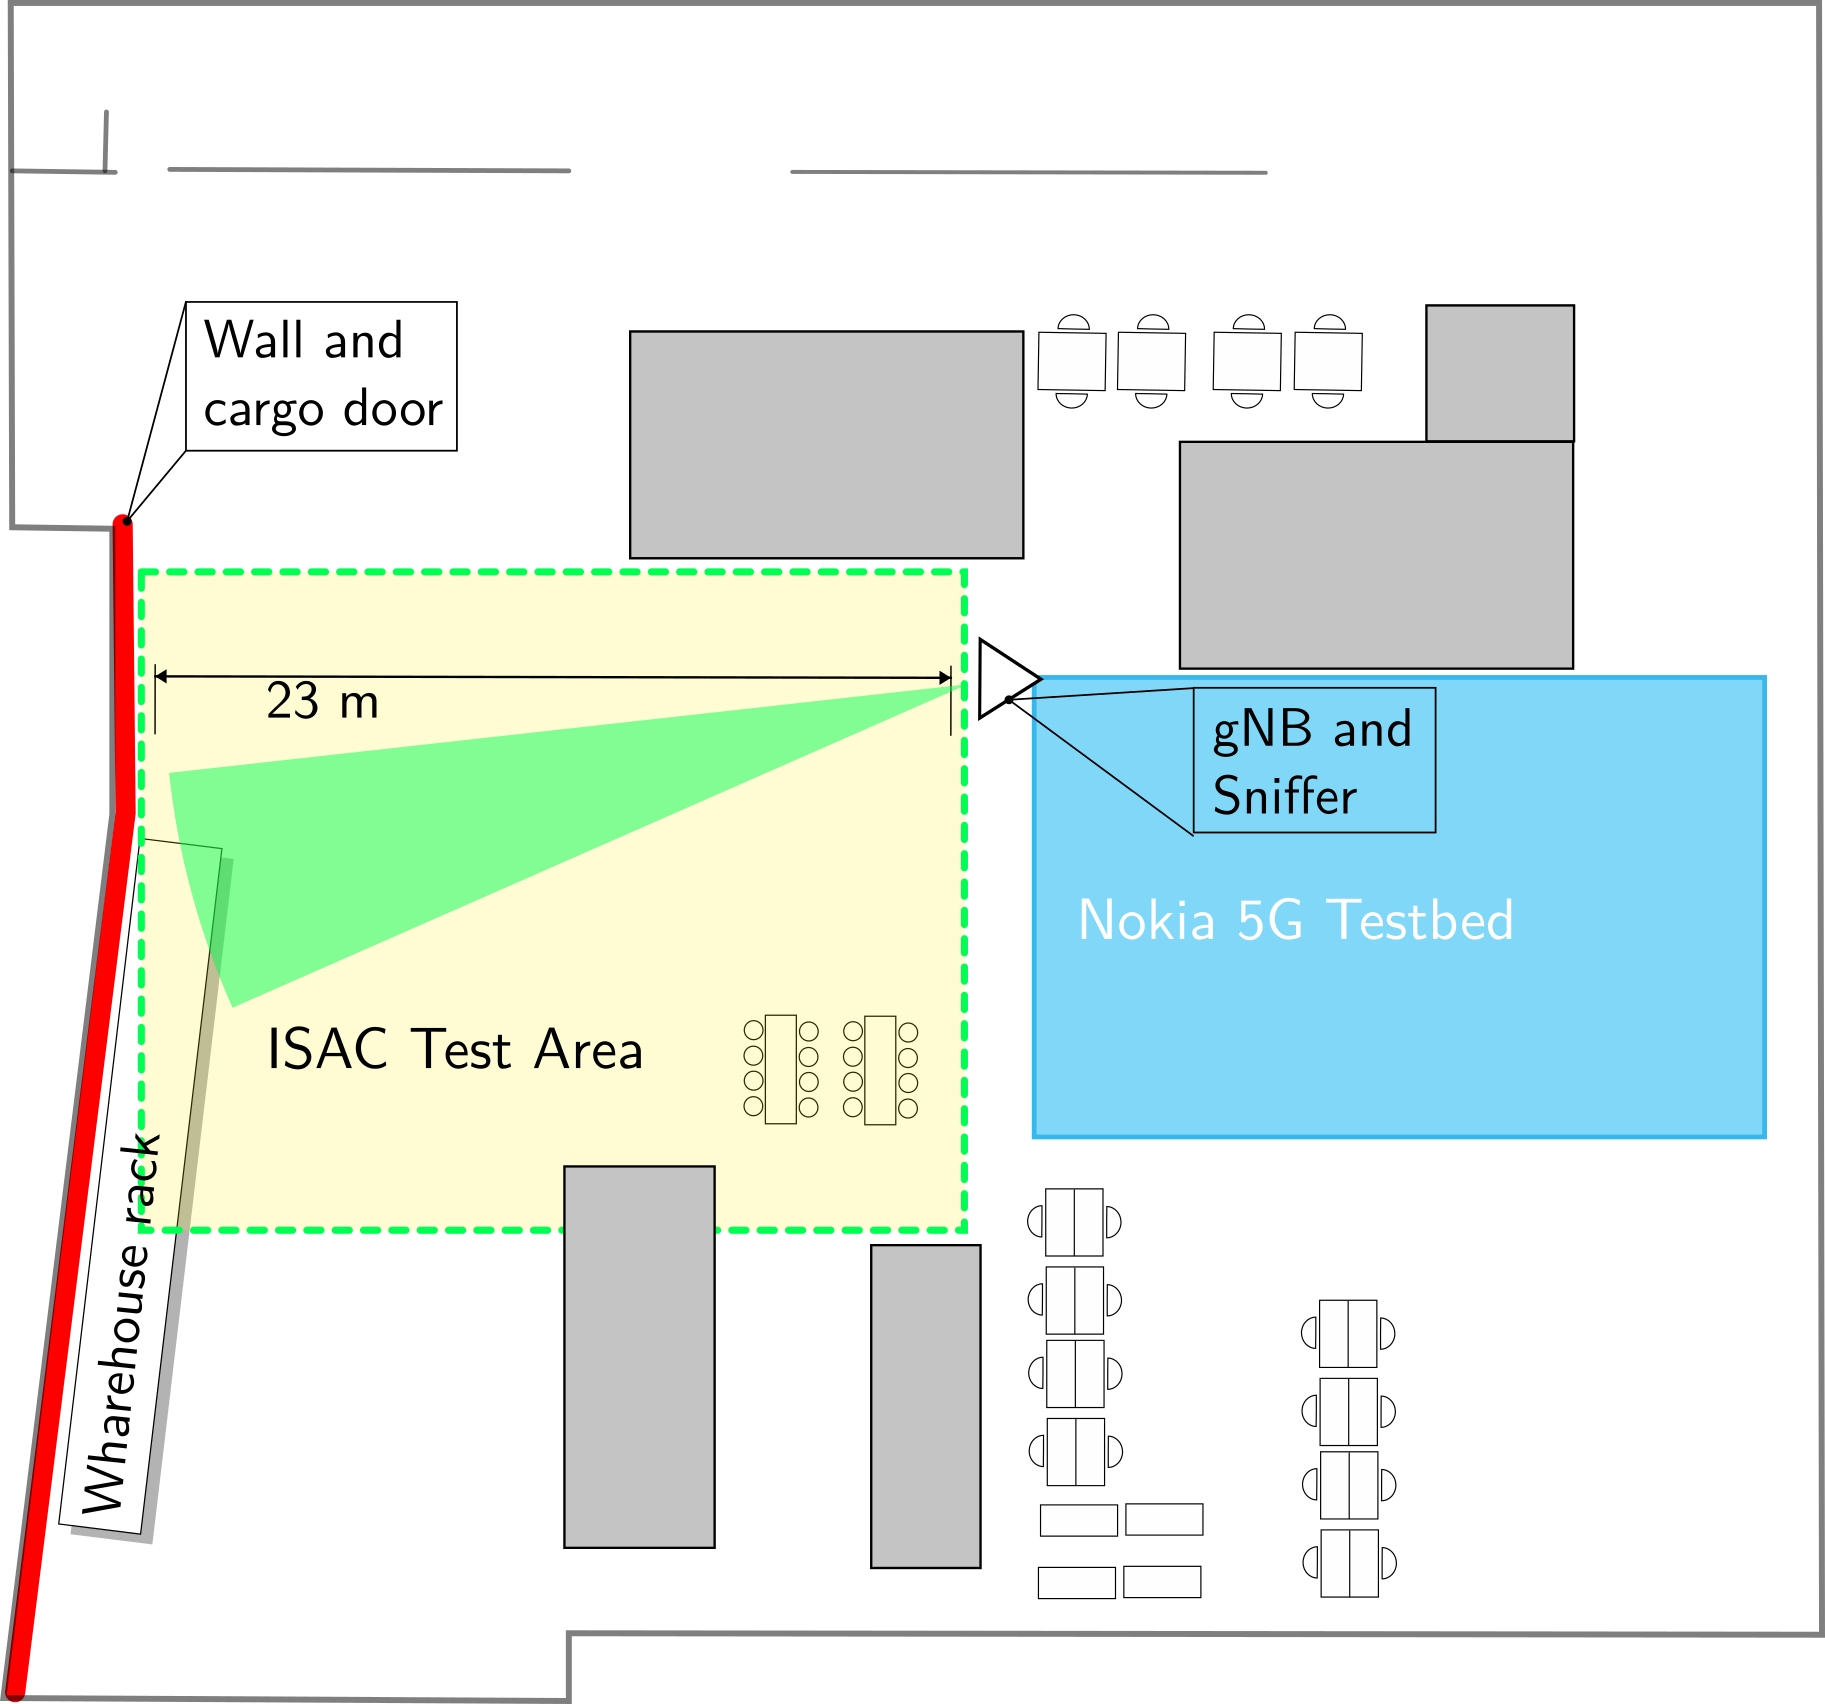
\includegraphics[width=.6\textwidth]{Images/Test1/arena_plan}
	\caption{Scheme of the PoC deployment layout in ARENA 2036, Stuttgart.}
	\label{fig:Test1_arena_plan}
\end{figure}


\begin{figure}[H]
	\centering
	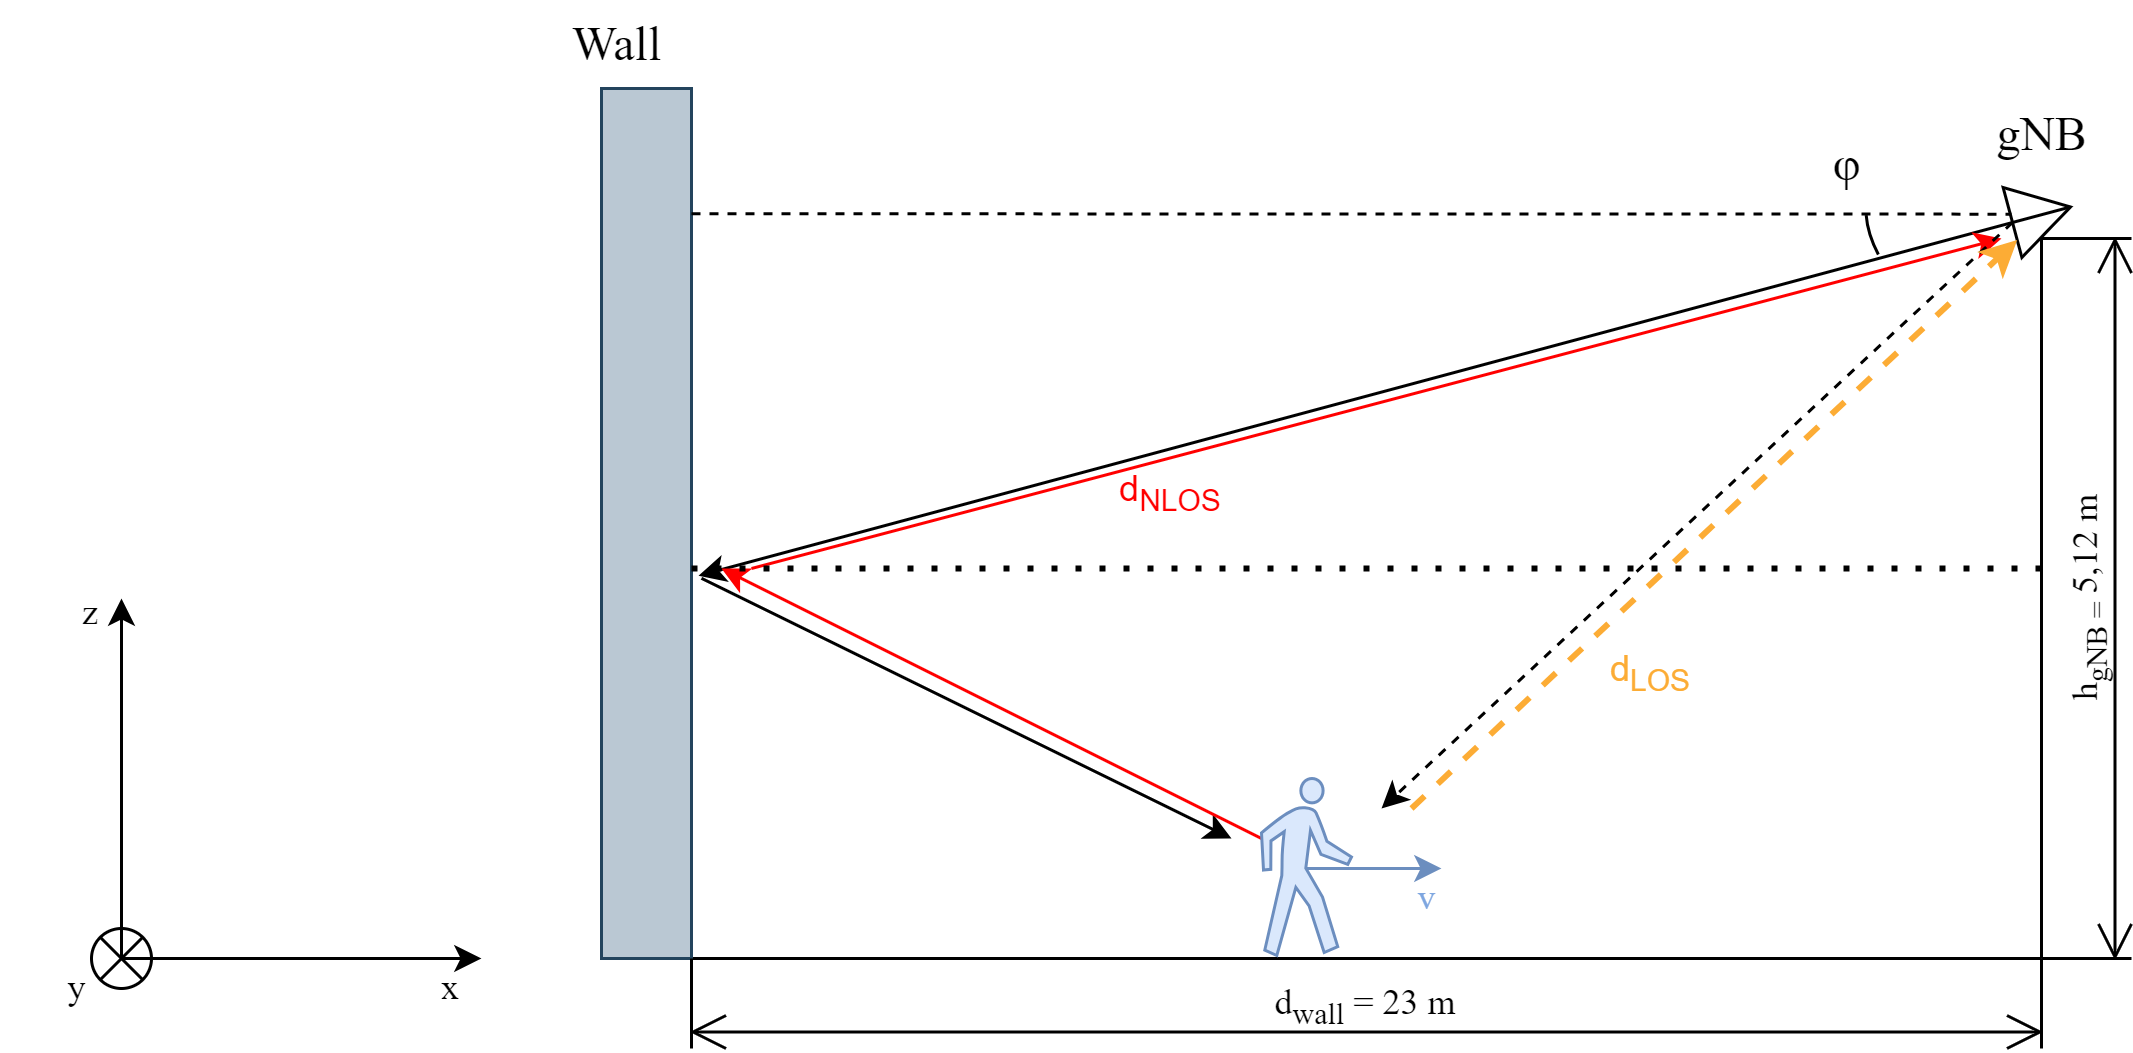
\includegraphics[width=1\textwidth]{Images/Test1/base-lateral_view_los_geometry}
	\caption{\small Lateral view of measurement scenario. NLOS return (red) is coupled with a LOS component (orange) generated from the secondary lobe.}
	\label{fig:Test1_base-lateral_view}
\end{figure}

\section{Measurement Scope: Detection Rate}

The radar system using OFDM can determine the range and radial speed of a target.\alert{ In this case with a fixed angle of arrival (AOA).} If an object moves azimuthally within the transmitted beam, it will appear static to the sensing system.

The test aimed to maximize the radial speed of the target to analyse the characteristics of the signal generated by its reflection.

During the initial measurement, the antenna boresight was directed perpendicular to the wall, while the target moved radially between the transmitter and reflector. The test subject moved towards the gNB and back multiple times in a straight line during the measurements.

\begin{figure}[H]
	\centering
	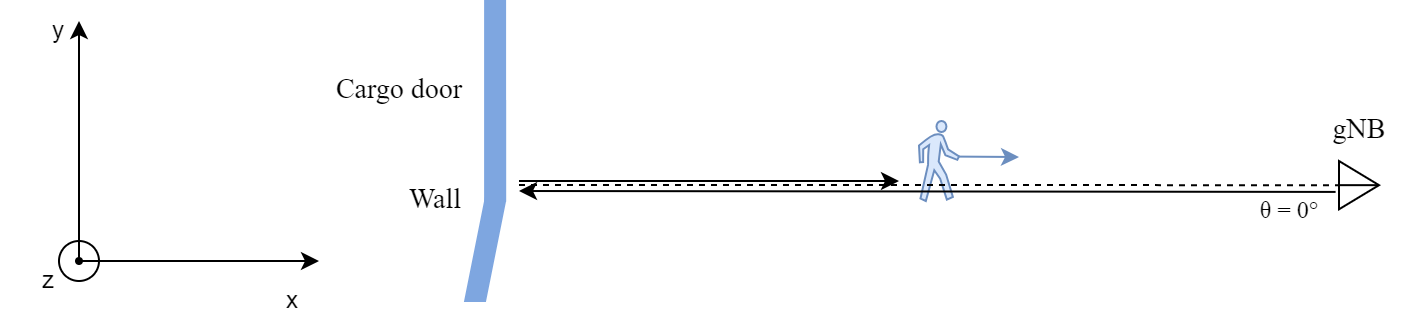
\includegraphics[width=1\textwidth]{Images/Test1/base-top_view}
	\caption{\small Top view of measurement scenario.}
	\label{fig:Test1_base-top_view}
\end{figure}


The beam elevation was chosen to be as high as possible to pass over the target and reflect on the wall, simulating a non-line-of-sight (NLOS) environment.

Due to the rather large beamwidth of the system, $\pm$7\textdegree\hspace{1pt} in azimuth and elevation, and its sidelobes, the measurement observed the presence of a LOS target return in addition to the expected NLOS one generated by reflection.

During the measurement, the direct component was always visible as no other obstacle was positioned in the scene. It was then decided to use this component and the knowledge of the geometry of the test area to obtain an estimate of the position and velocity of the NLOS return. This estimate was used to check if any of the detected peaks corresponded to the moving target.
The direct target return provided additional information, which was then used as ground truth to determine the correct position of the person within the test area.
Figures \ref{fig:Test1_base-lateral_view} and \ref{fig:Test1_base-top_view} depict a scheme of the measurement.

Considering the processing scheme proposed in Section \ref{sec:nlos_proc_pipeline}, the periodogram was processed differently after separation in the regions corresponding to LOS and NLOS conditions.
A standard strongest peak search is performed for the LOS region, while multiple peak detection is conducted in NLOS, where only the five strongest peaks were considered. This assumption was made since the test was conducted in a single target scenario and a single NLOS return is expected.
Accurate range and velocity measurements are obtained after interpolation of each peak with the adjacent bins.

\begin{itemize}
	\item Speed of the NLOS component was estimated as:
	$$ \hat{v}_{\text{NLOS}} = -v_{\text{LOS}}$$
	since the direct and reflected beams will hit the target from the opposite direction, hence measuring the target's speed with opposing sign.
	\item Range of the NLOS component was estimated considering the model in Figure \ref{fig:Test1_base-lateral_view} as:
	$$ \hat{d}_{\text{NLOS}} = 2 d_{\text{wall}} - d_{\text{LOS}}\cdot \cos{(\arctan{\left(\frac{h_{\text{gNB}}}{d_{\text{LOS}}}\right)})}$$
\end{itemize}


\textit{Detection rate} was defined as the metric used to evaluate the experiment: if the speed and range of the NLOS return matched the expected values calculated from the LOS data, detection was considered positive.
The detection rate was then obtained as the ratio between the number of frames in which the NLOS component was above threshold, and the total number of frames in which the LOS component was detected.


\begin{equation*}
	\text{Detection rate} = \frac{\text{frames with NLOS}}{\text{frames with LOS}}
\end{equation*}

Due to the multiple reflections, the NLOS return presented considerably smaller power compared to LOS.
This meant that due to the presence of large clutter returns and their sidelobes, this return is not necessarily the strongest one in the NLOS region of the periodogram.
Detection rate was hence evaluated comparing the five strongest returns in NLOS with the estimated position of the target.


\section{Observation on detection rate of a strong reflector}

	\begin{figure}[H]
	\centering
	
	\subfloat[\footnotesize Metal cabinet moving towards gNB, linear scale.\label{fig:Test1_metal_lin}]{%
		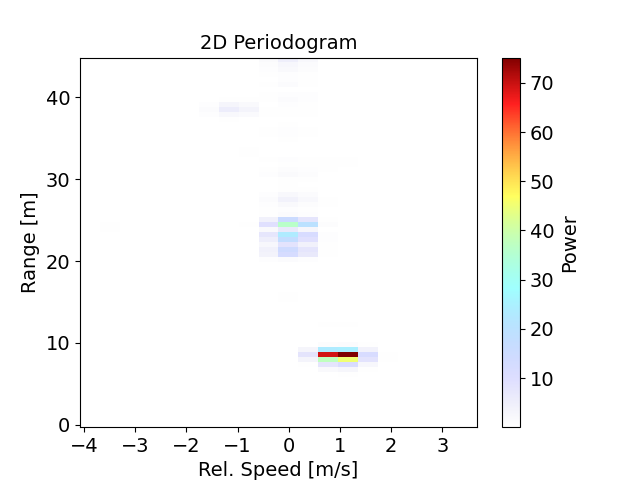
\includegraphics[scale=0.45]{Images/Test1/per_strong_ref/linear_1frame_dec_CRAP.png}%
	}\hfill
	\subfloat[\footnotesize Metal cabinet moving towards gNB, power in dB.\label{fig:Test1_metal_db}]{%
		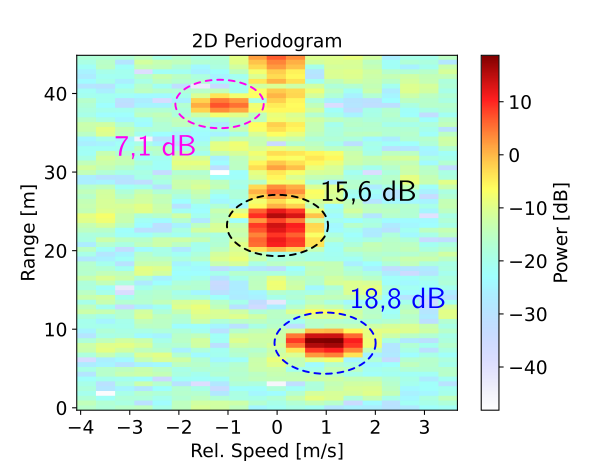
\includegraphics[scale=0.45]{Images/Test1/per_strong_ref/db_1frame_dec_CRAP_labelled_text22.png}%
	}\hfill
	\subfloat[\footnotesize Human target walking towards gNB, power in dB.\label{fig:Test1_metal_human-baseline}]{
		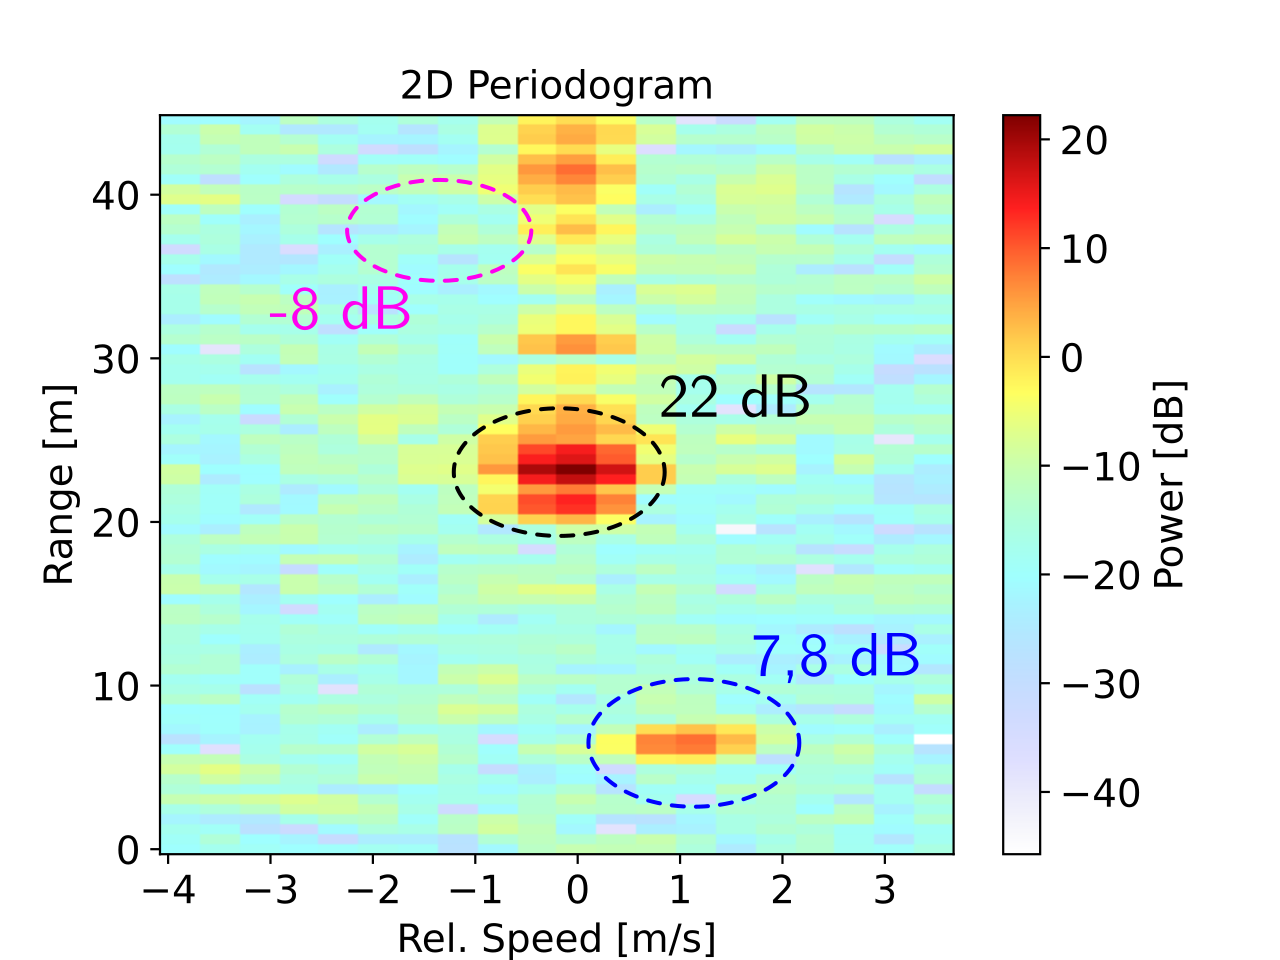
\includegraphics[scale=0.45]{Images/Test1/per_strong_ref/db_1frame_dec_CRAP_HUMAN_labelled_text22.png}
	}
	\caption[]{\small Comparison of periodograms from sensing acquisitions obtained in NOKIA's industrial test facility.
		All the periodograms are obtained by processing a single decimated CSI frame (24 symbols), after applying clutter removal with CRAP.
		Periodograms \subref{fig:Test1_metal_lin} and \subref{fig:Test1_metal_db} show the returns obtained with the metal cabinet. The NLOS return (purple) is clearly separated from the underlying noise floor, even when processing only 24 symbols. On the contrary the NLOS component generated from the human target in \subref{fig:Test1_metal_human-baseline}, requires for a considerably higher processing gain to be detected reliably.}
	\label{fig:Test1_metal-human_comparison}
	\end{figure}
	
The first measurement was performed with the strong reflector, which represented an ideal scenario. 
Figure \ref{fig:Test1_metal-human_comparison} illustrates the comparison between the human and the metal cabinet cases. 
Even when decimating the single CSI matrix, translating a 15 dB loss in processing gain, the NLOS component of the metal cabinet can be easily identified when moving.

The detection rate test displayed in figure \ref{fig:Test1_detect_rate_strong_ref} shows that the passive reflector, thanks to its significantly larger radar cross section, is clearly identified while it is moving and has stronger power compared to reflected clutter returns.

Passing the NLOS measurements to a Kalman filter it was possible to track the target in the range/Doppler plane, as shown in figure \ref{fig:Test1_kf_track_strong_ref}. This result is to show that one of the main limitation of NLOS signals is the strength of the target return. Objects with large RCS are easier to separate from the noisy background and the effect of fading and obstruction is relatively small.

\begin{figure}[H]
	\centering
	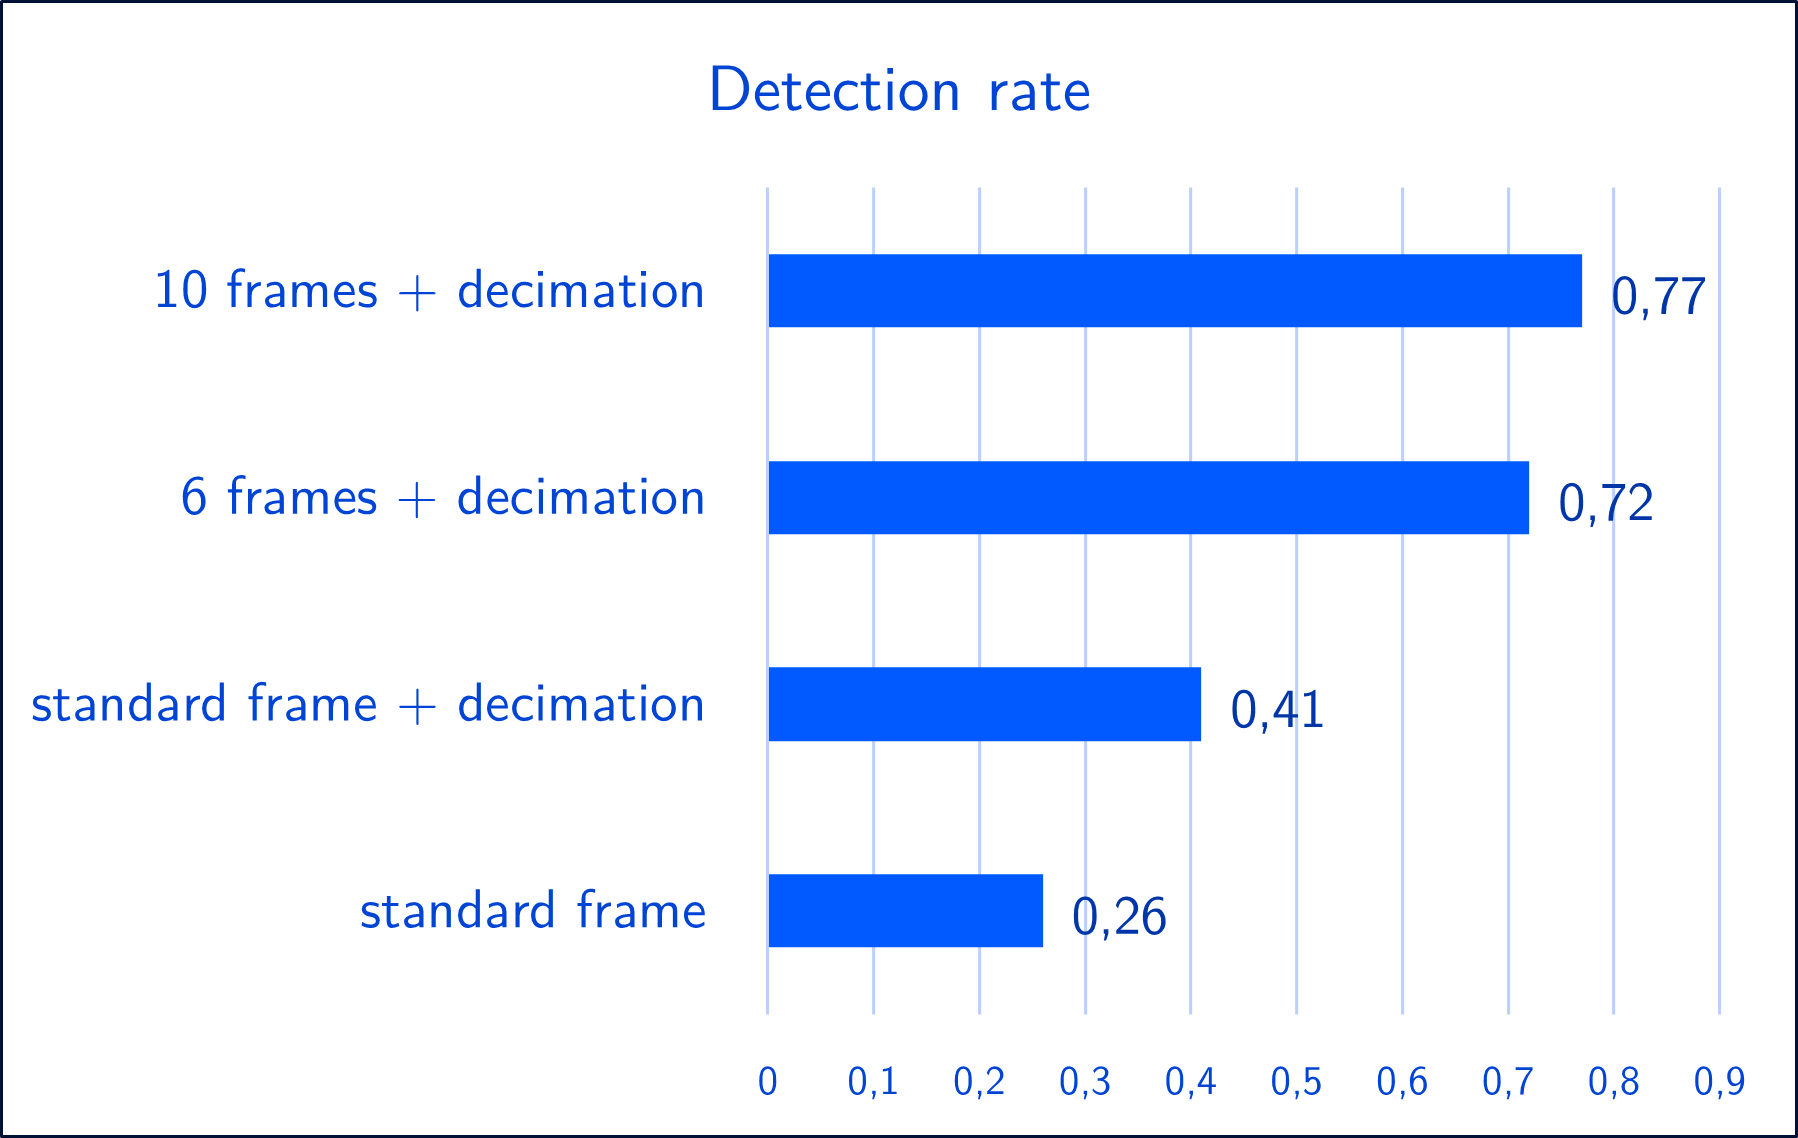
\includegraphics[width=0.55\textwidth]{Images/Test1/detect_hist/detect_hist_cabinet_LMsans.png}
	\caption{\small Detection rate observed for passive metal reflector target in mixed LOS/NLOS measurement.}
	\label{fig:Test1_detect_rate_strong_ref}
\end{figure}



\begin{figure}[H]
	\centering
	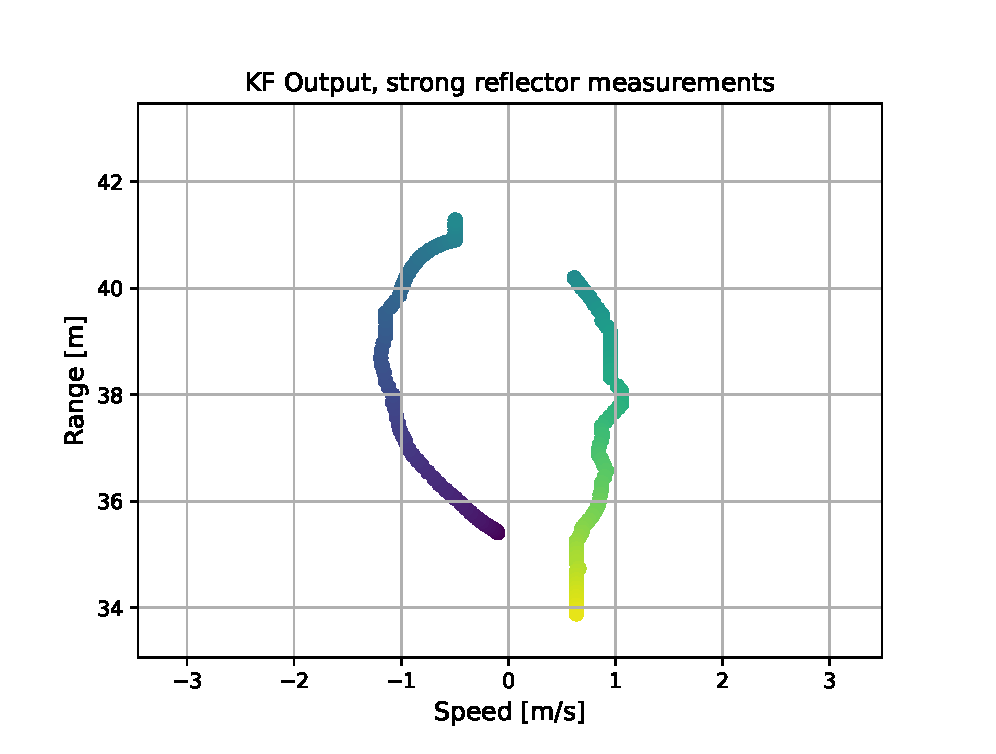
\includegraphics[width=0.55\textwidth]{Images/Test1/kf_track.eps}
	\caption{\small KF track of the target in the range/speed plane. Track is interrupted when the target stops and changes direction.}
	\label{fig:Test1_kf_track_strong_ref}
\end{figure}


\subsection{Human target detection}

The detection rate for measurements with a walking actor was obtained using the various frame processing strategies presented in chapter \ref{chap:TDD pattern of the OFDM frame}. To increase time-aperture, subsequent frames were combined, and the window processing stride was set to be lower than the number 
of frames, allowing for more target updates.

Clutter removal was performed using CRAP to ensure precise estimation of the expected target position in NLOS conditions. In contrast, periodograms generated with the ECA-C technique showed the NLOS component to be well separated from the underlying noise floor, but the estimated position did not correspond with the measured one, making the detection test difficult. Comparison of a sample radar update after CRAP and ECA-C is shown in Figure \ref{fig:Test1_huma_crap-ecac}.

	\begin{figure}[H]
	\centering
	
	\subfloat[Periodogram after applying CRAP.\label{fig:Test1_mhuman_crap}]{%
		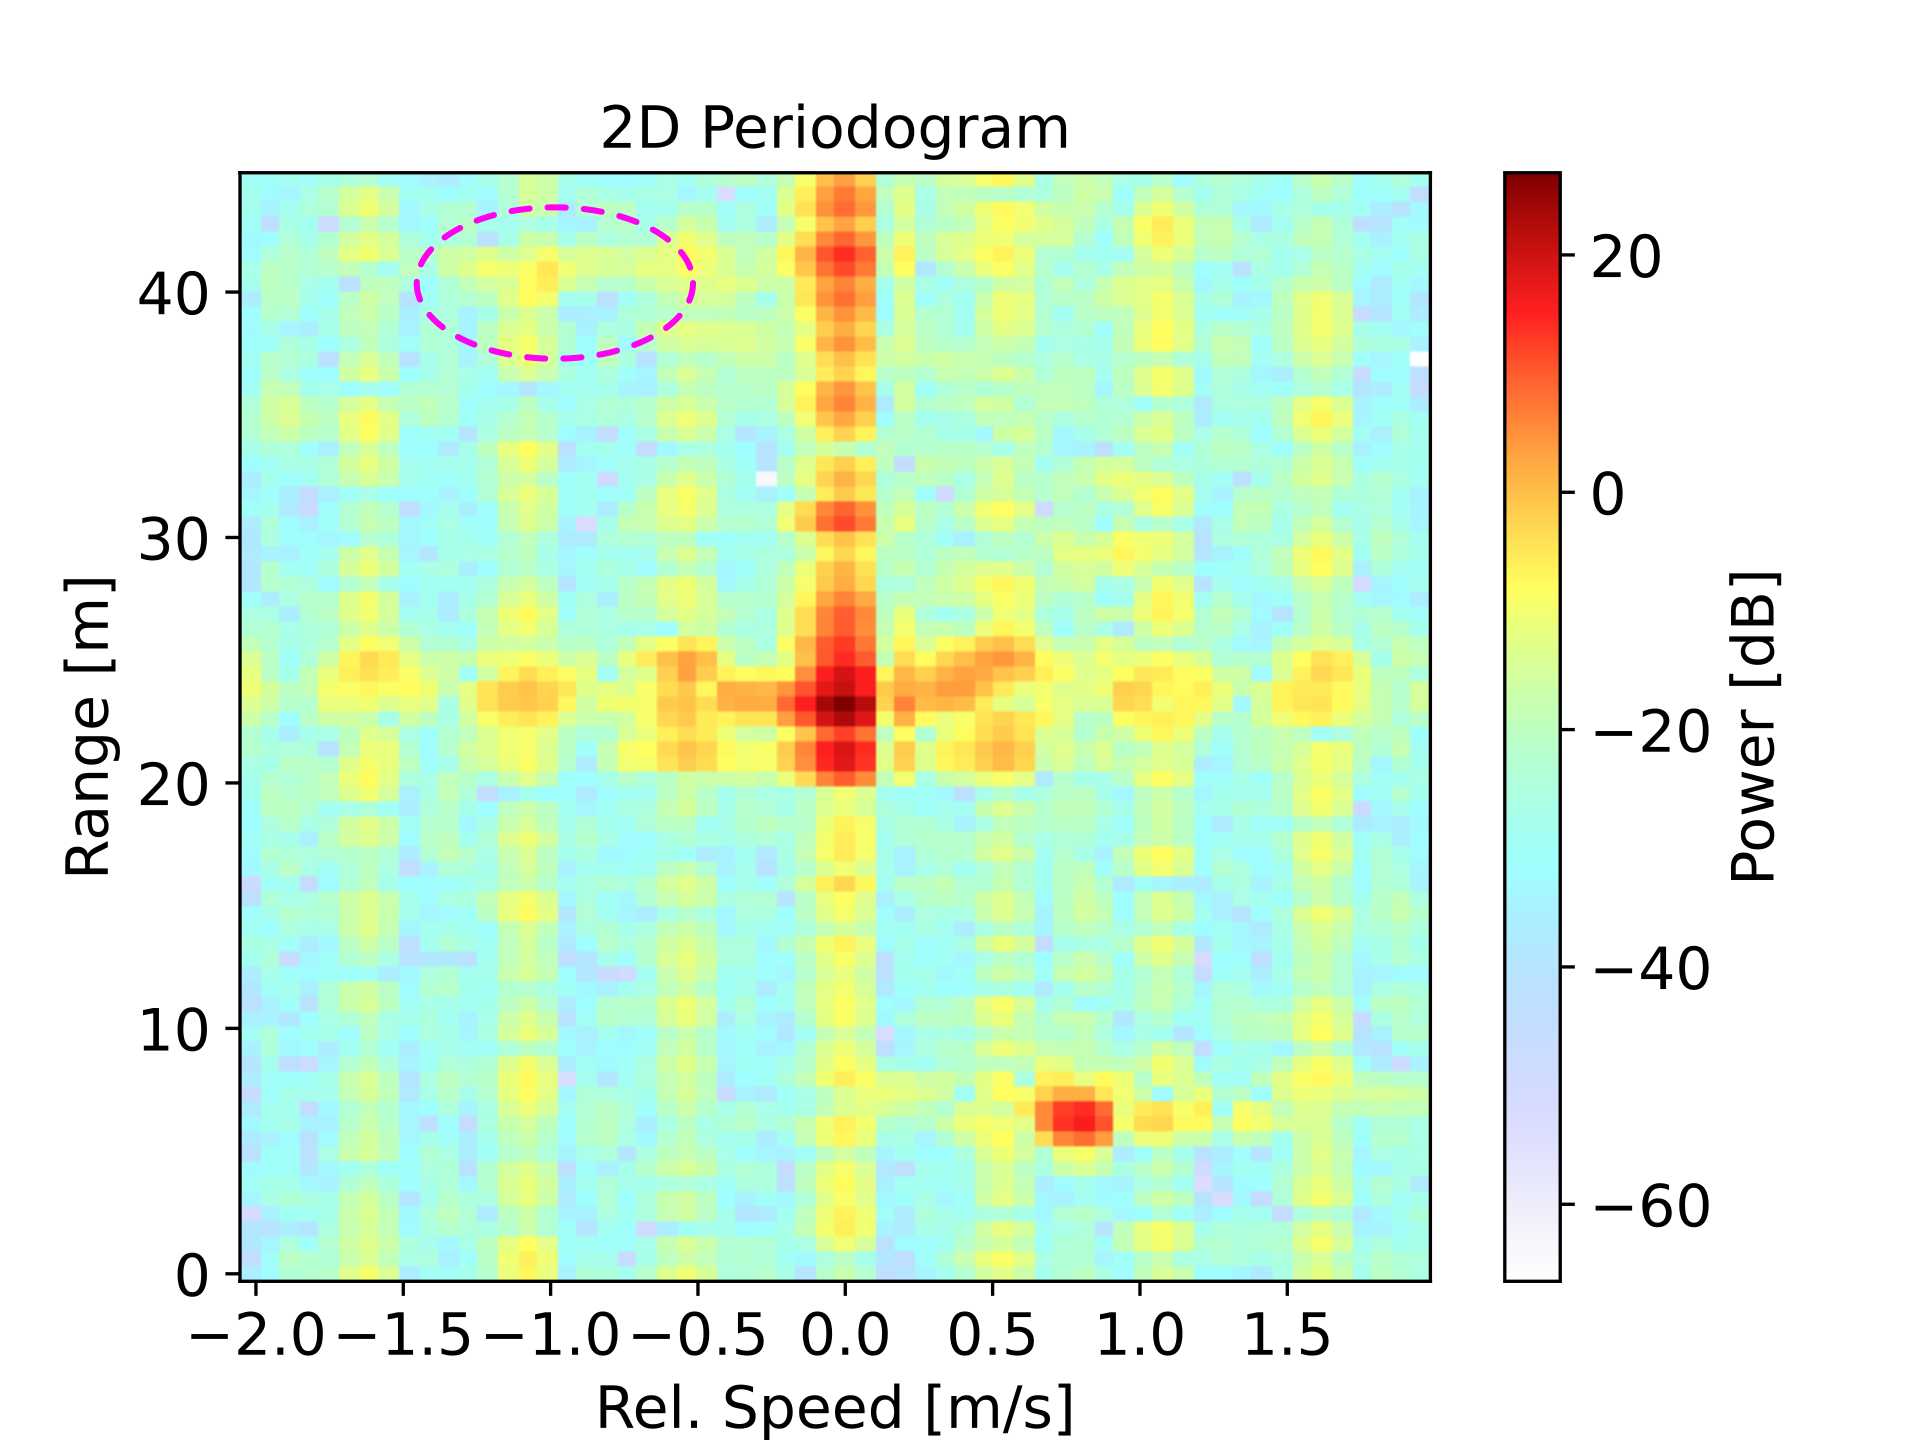
\includegraphics[scale=0.45]{Images/Test1/Human_crap_ecac/crap_labelled.png}%
	}\hfill
	\subfloat[Periodogram after applying ECA-C.\label{fig:Test1_mhuman_ecac}]{%
		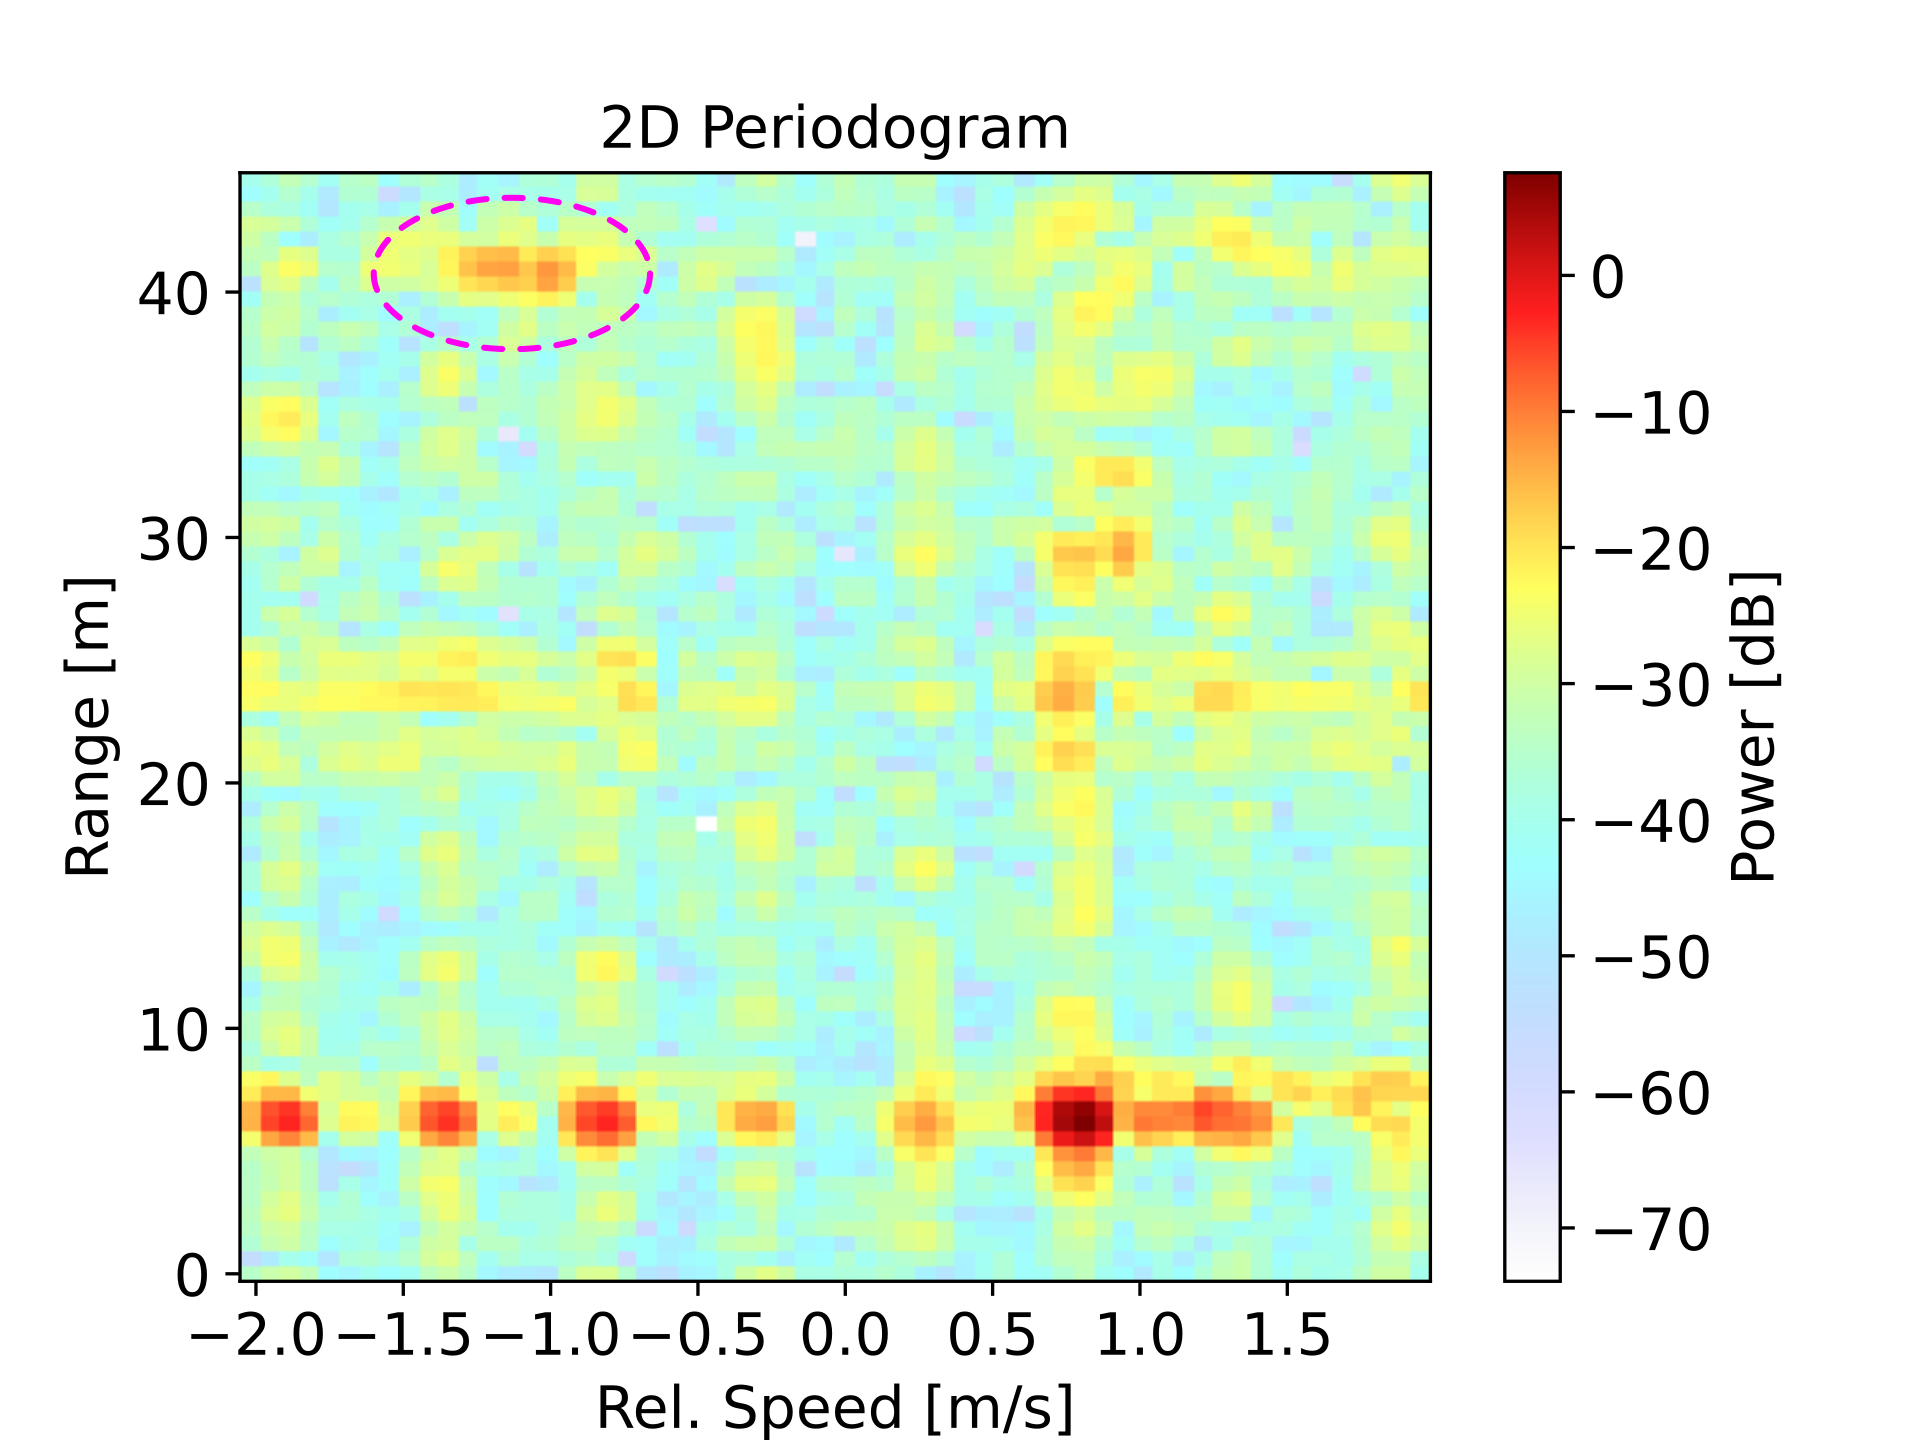
\includegraphics[scale=0.45]{Images/Test1/Human_crap_ecac/ecac_labelled.png}%
	}
	\caption[]{\small Comparison of periodograms from sensing acquisitions obtained in NOKIA's industrial test facility.
		Periodogram obtained by processing 6 consecutive frames.
		In \subref{fig:Test1_mhuman_crap} the NLOS return presents a single, but its power is comparable with the one of the nearby artefacts. In \subref{fig:Test1_mhuman_ecac} the return is distorted in two peaks, moreover the sidelobes of the LOS component are enhanced and appear as ghost targets.}
	\label{fig:Test1_huma_crap-ecac}
\end{figure}




Target detection was carried out by considering the 'n'-strongest peaks and comparing them against the LOS data. If any of the observed non-line-of-sight (NLOS) peaks corresponded to the target, then the detection was positive.

\begin{figure}[H]
	\centering
	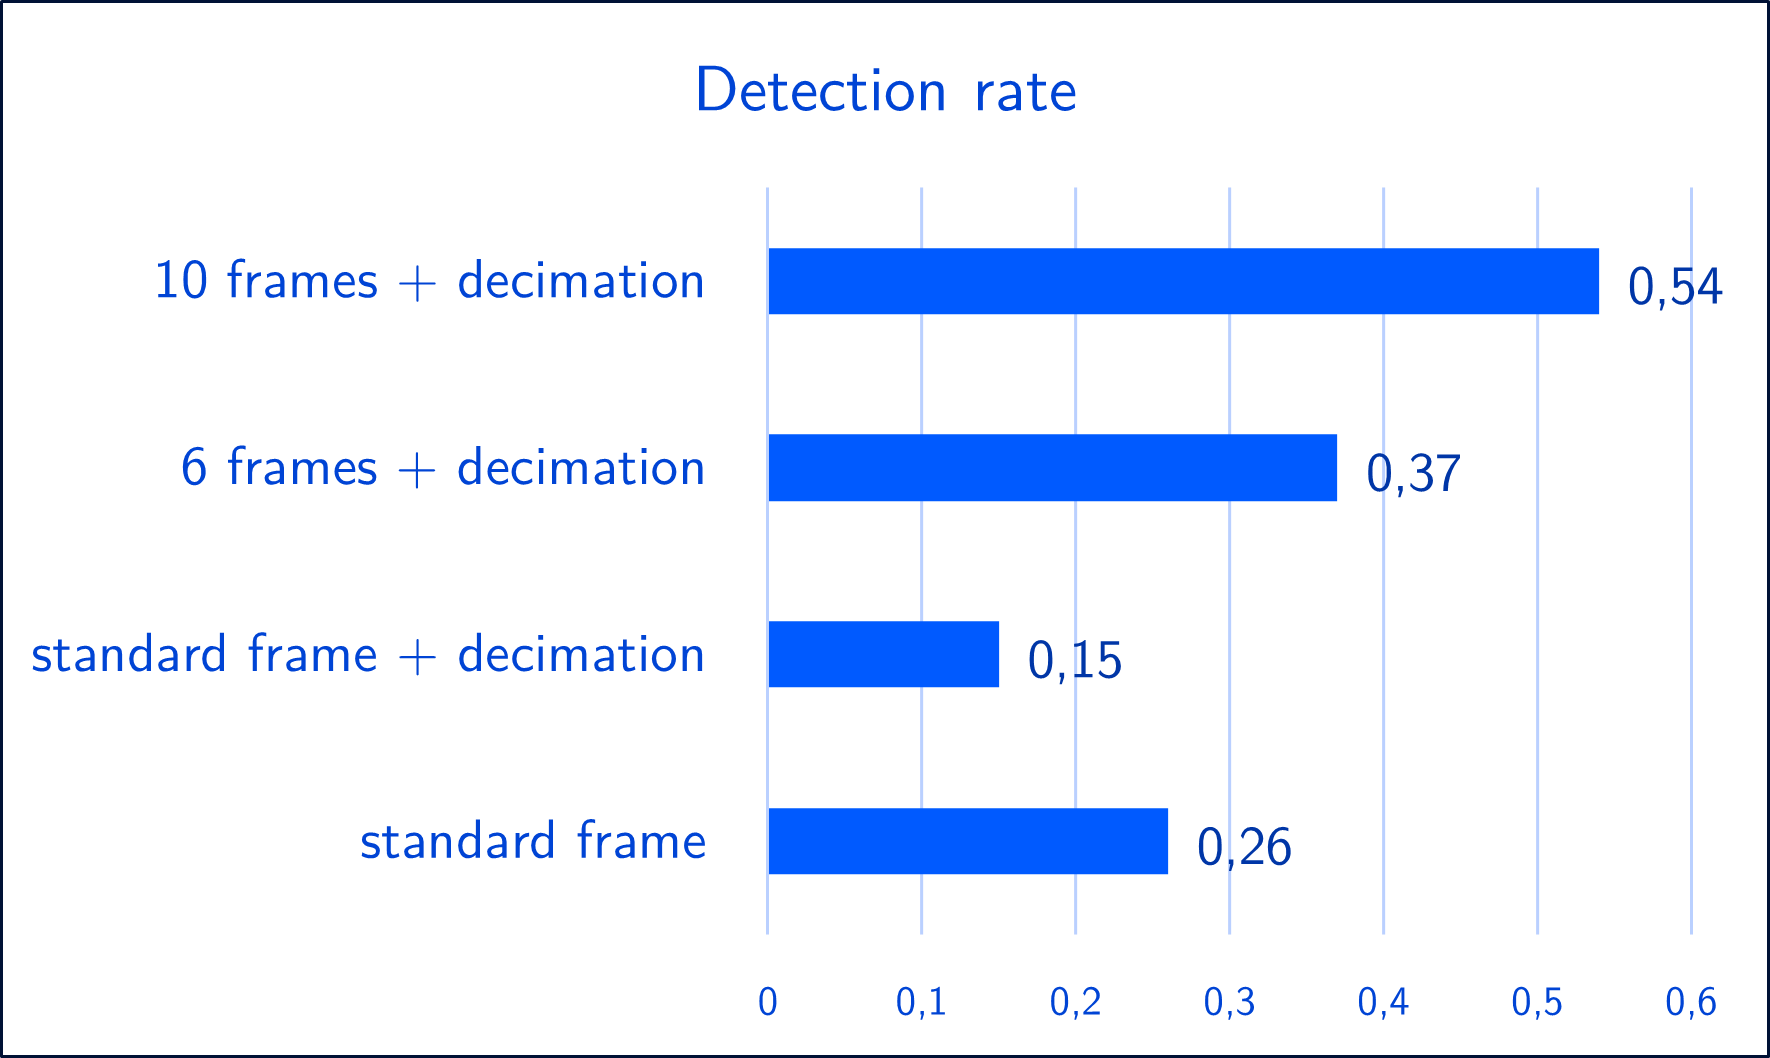
\includegraphics[width=0.7\textwidth]{Images/Test1/detect_hist/detect_hist_human_LMsans.png}
	\caption{Detection rate observed for human target in mixed LOS/NLOS measurement. Clutter removal performed with CRAP.}
	\label{fig:Test1_detect_hist}
\end{figure}

Increasing the time-aperture significantly improved the detection rate due to the larger SNR.

In most cases, the NLOS target return was not the strongest due to lower peak power compared to noise. Additionally, when increasing the time aperture, spectral artefacts were present.
Target returns occasionally suffered from channel fading, causing their power to change between consecutive updates. In contrast, artefacts' power remained relatively constant and proportional to the number of processed frames.

The detection rate was observed throughout the entire measurement, including frames where the target changed direction and was either static or presented a low-speed component. However, processing these time instants may have masked the NLOS component with clutter and resulted in a negative detection. Therefore, the effective detection rate, which is measured only when the target is in motion, is likely to be higher.


%TODO: change subsection title
\subsubsection{Moving average of detection rate}

Figure \ref{fig:Test1_moving_avg} shows the average detection rate over 10 consecutive updates. It is evident that the detection rate is above 80\% for several consecutive 10-update intervals when the target is in motion and therefore well separated from the clutter region.


Although this measure was obtained in a controlled single-target scenario, it opens the possibility of detecting the presence of non-line-of-sight (NLOS) moving targets without relying on additional ground truth data.


% TODO: change picture with higher resolution one, maybe solved
\begin{figure}[H]
	\centering
	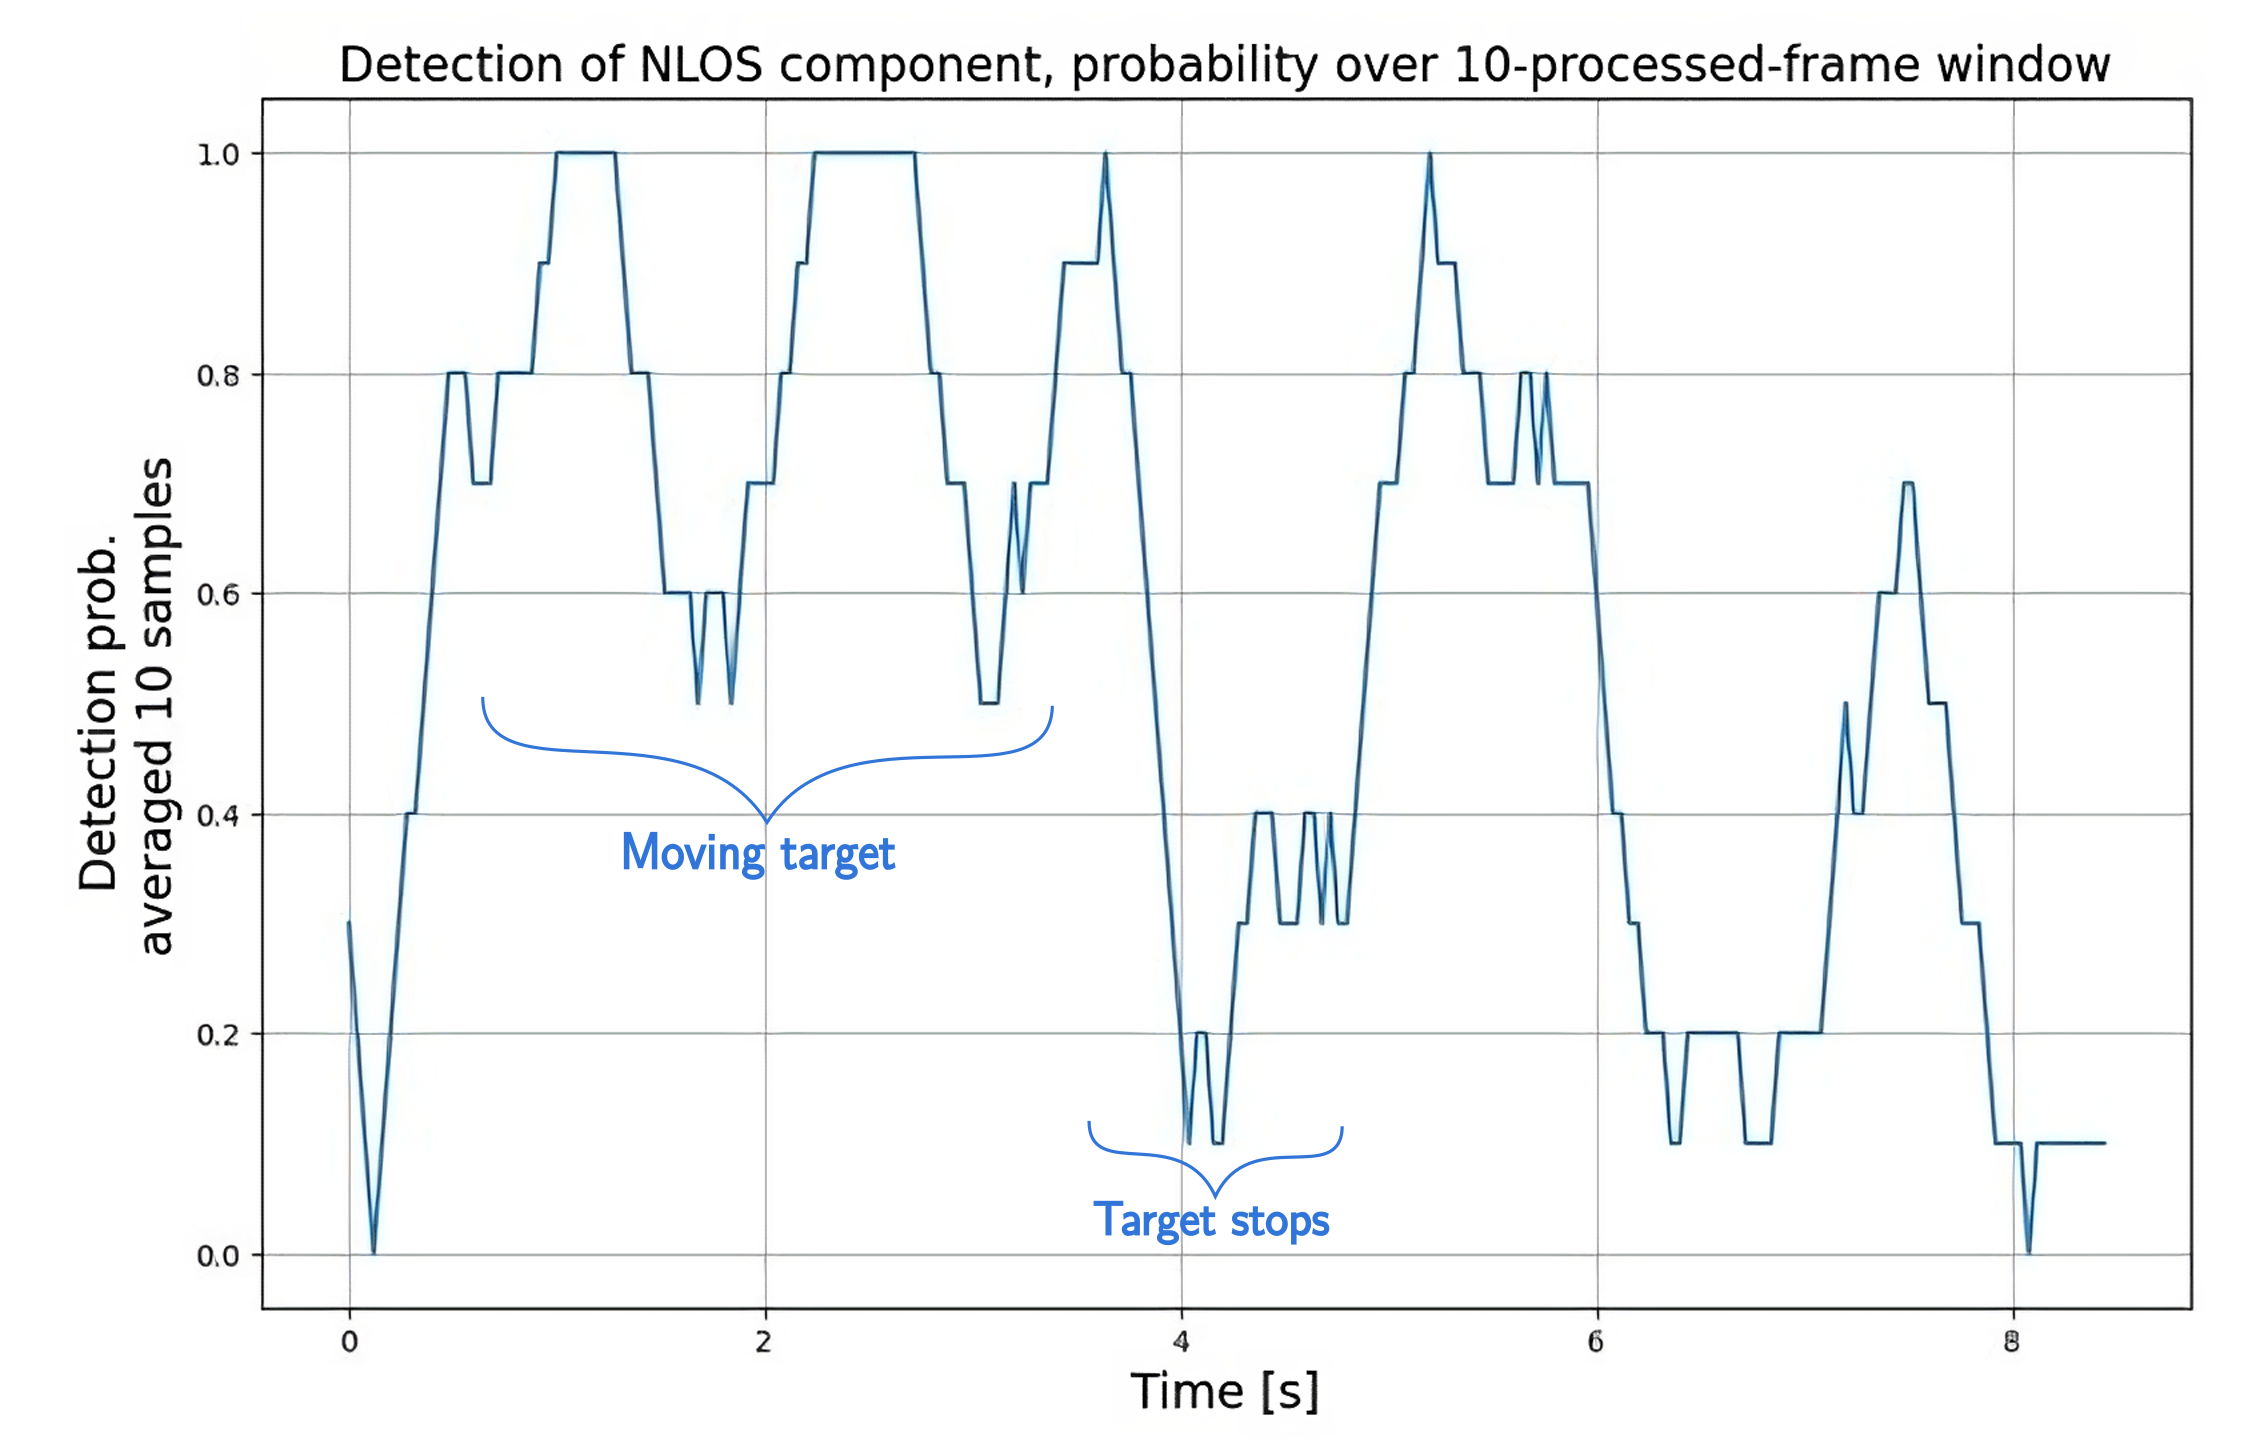
\includegraphics[width=0.7\textwidth]{Images/Test1/moving_avg-transformed_wtext}
	\caption{Detection rate observed for human target in mixed LOS/NLOS measurement.}
	\label{fig:Test1_moving_avg}
\end{figure}


\subsubsection{Detection rate with separate clutter removal for NLOS}

Figure \ref{fig:Test1_huma_crap-ecac} illustrates the tradeoffs between using CRAP and ECA-C for clutter removal. It can be seen that CRAP is ideal for line-of-sight (LOS) targets, while the power of the non-line-of-sight (NLOS) return is reduced to a level similar to the Doppler artefacts.

On the other hand, ECA-C introduces distortion and loss of information at zero speed, which is not suitable for any use case requiring LOS. In NLOS the static bin of the periodogram is discarded anyway, while the target return can be easily distinguished from the underlying noise floor.

The detection rate was tested using CRAP and ECA-C for the LOS and NLOS regions respectively, and the results are shown in Figure \ref{fig:Test1_moving_avg}.
This approach improved detection when the target was in motion.

\begin{figure}[H]
	\centering
	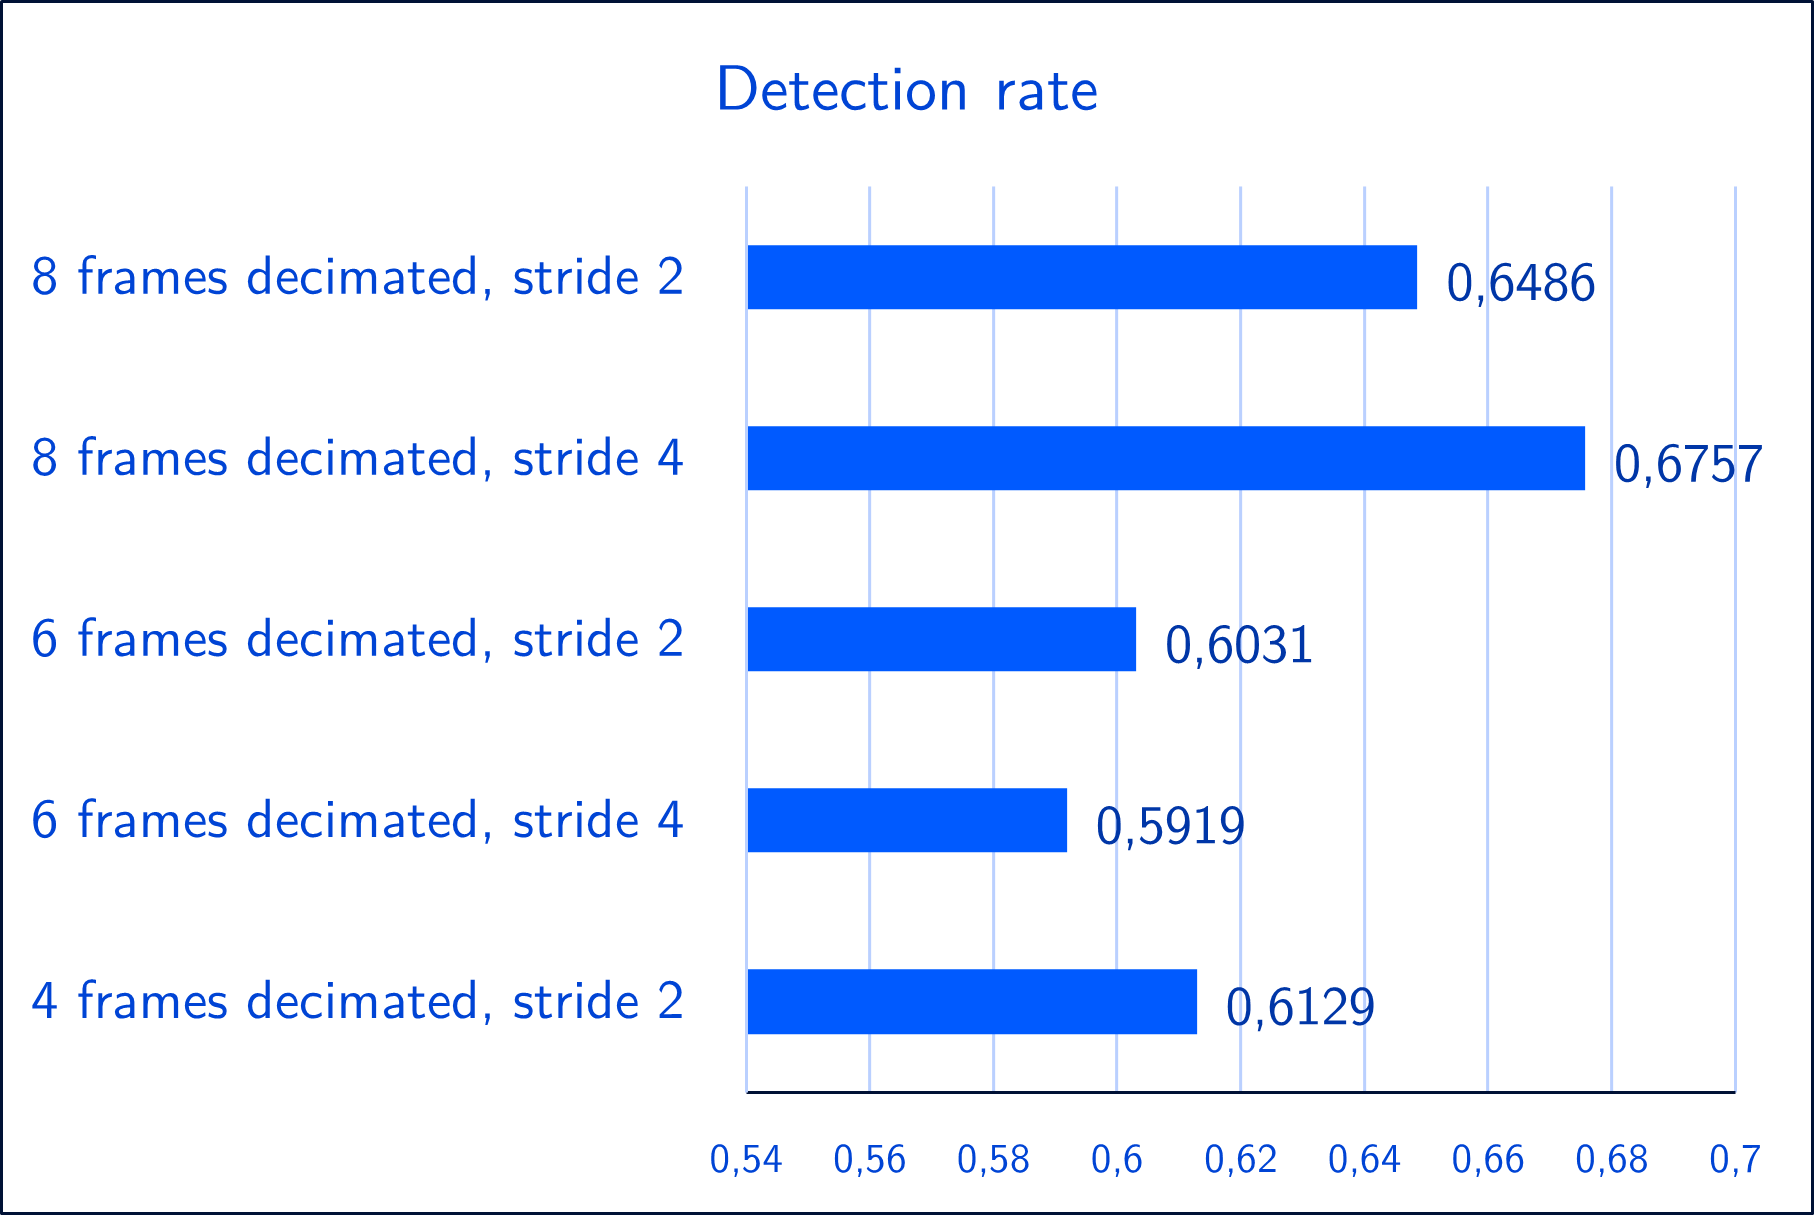
\includegraphics[width=0.7\textwidth]{Images/Test1/detect_hist/detect_hist_human_ECAC_LMsans.png}
	\caption{\small Detection rate observed for human target in mixed LOS/NLOS measurement. Clutter removal performed with ECA-C for the NLOS region and CRAP for the LOS.}
	\label{fig:Test1_detect_hist_crap-ecac}
\end{figure}


The measurement was not affected by the loss of information due to ECA-C when the target was static, as the bins of the periodogram corresponding to null speed were discarded regardless.

The moving average of the detection probability is shown in Figure \ref{fig:Test1_mov_avg_crap_ecac}.
It is evident that the detection from seconds 5 to 7 is significantly improved when compared to using only CRAP.
However, this approach incurs a high computational cost as both clutter removal methods need to be applied to each OFDM frame separately.

\begin{figure}[H]
	\centering
	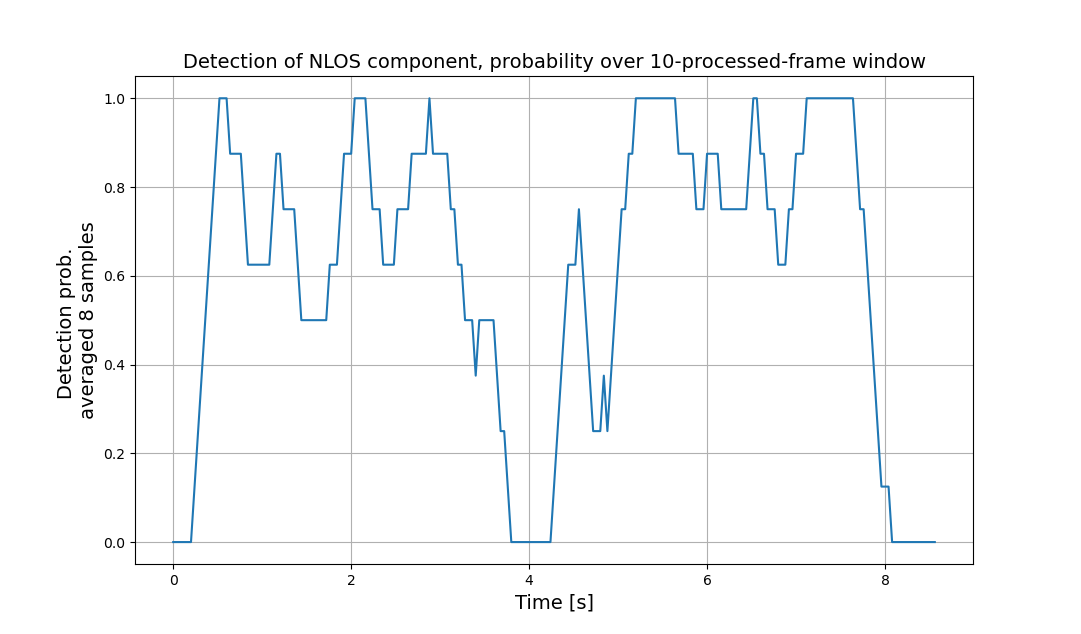
\includegraphics[width=0.8\textwidth]{Images/Test1/ECAC_CRAP_mixed/movavg_6frames_mixedecac-crap_stride4_exp_thresh.png}
	\caption{\small Detection rate observed for human target in mixed LOS/NLOS measurement. Clutter removal performed with ECA-C for the NLOS region and CRAP for the LOS.}
	\label{fig:Test1_mov_avg_crap_ecac}
\end{figure}
